%% This is an example first chapter.  You should put chapter/appendix that you
%% write into a separate file, and add a line \include{yourfilename} to
%% main.tex, where `yourfilename.tex' is the name of the chapter/appendix file.
%% You can process specific files by typing their names in at the 
%% \files=
%% prompt when you run the file main.tex through LaTeX.

\singlespacing{

\chapter{Implementation}

\href{http://git.amandaghassaei.com/KinematicCA/}{AmoebaCAD} is a 3D CAD and simulation tool, based off the ideas from Chapters \ref{chap:CAD} and \ref{chap:functionSim}.  In this tool, users construct assemblies of functional primitives and simulate their electronic and mechanical behaviors.  This chapter introduces information about the software implementation of Amoeba.

\section{Javascript/WebGL}

AmoebaCAD was written in HTML5/JavaScript and currently hosted online.  I chose the web as a development platform for this project because it allows easier access to the code than any other platform.  Though user studies are not a component of this work, there is a long history of communities of users building things in sandbox environments that surpass anything the developers were able to imagine.  There is a lot of talent beyond the immediate neighborhood of CBA, and I'd like to try to make this codebase accessible to anyone interested in exploring the design space around digital materials.\\

The web app was written with the following dependencies:
\begin{itemize}
\setlength\itemsep{0em}
\item \href{http://threejs.org/}{Three.js} is a library containing lots of useful classes for interacting with WebGL without getting bogged down in the details or sacrificing too much in performance.
\item \href{http://requirejs.org/}{RequireJS} is a framework for asynchronously loading JavaScript modules and dependencies.
\item \href{http://backbonejs.org/}{Backbone.js} is a framework for managing UI events and giving structure to complex, interactive applications.
\item \href{https://jquery.com/}{JQuery} is a library that handles interactions between HTML and Javascript and help maintain cross browser support of UI elements.
\item \href{http://underscorejs.org/}{Underscore} is a library with lots of useful functions for dealing with arrays and JavaScript objects.  Underscore also provides templating for Backbone.
\end{itemize}

\begin{figure}
  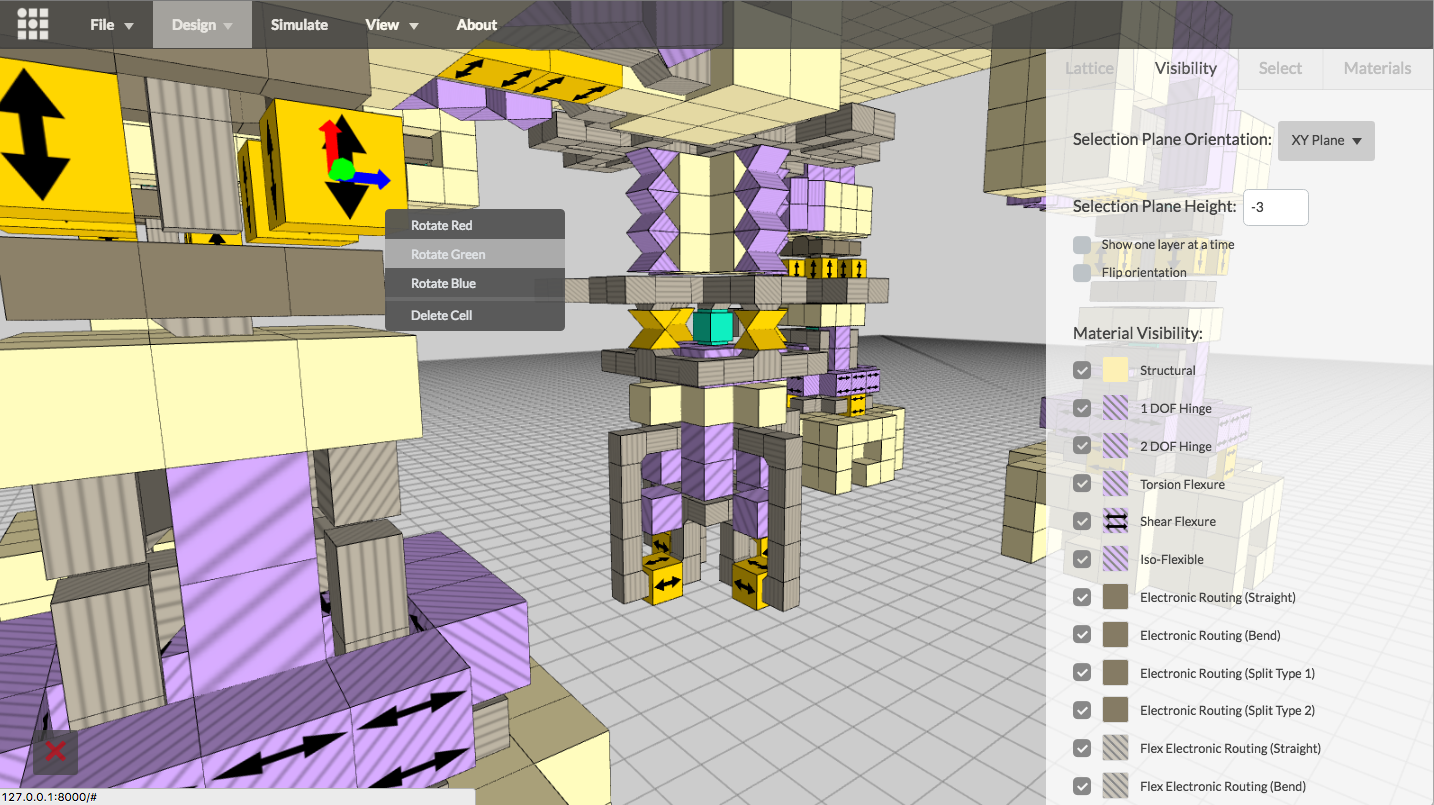
\includegraphics[width=\linewidth]{rotationGUI.png}
  \caption{A schematic diagram of a robotic "pick and place" in AmoebaCAD.  Cell rotation GUI allows anisotropic cells to be oriented in any direction.}
  \label{fig:rotationGUI}
\end{figure}

\begin{figure}
  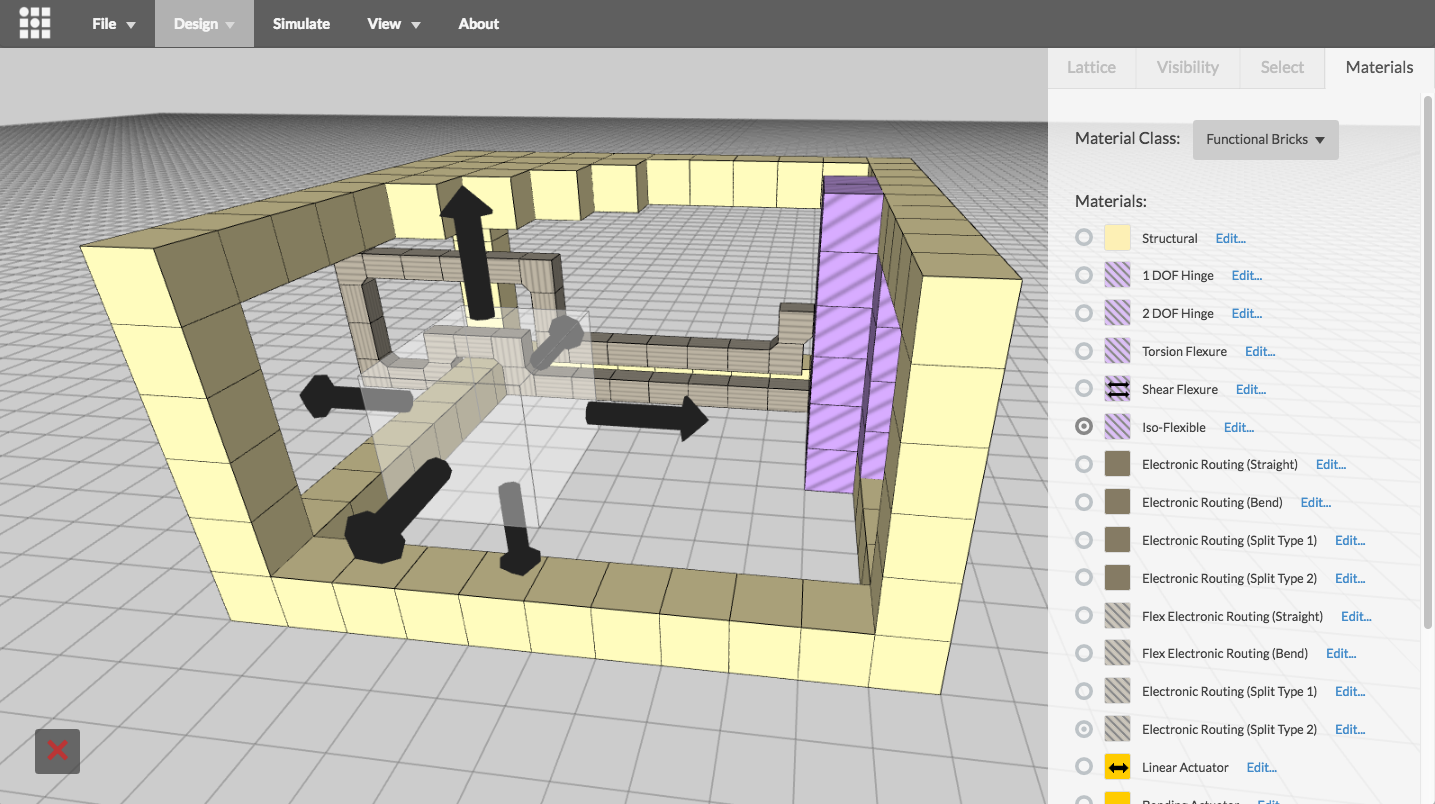
\includegraphics[width=\linewidth]{selectiontoolGUI.png}
  \caption{3D selection tool allows for bulk cell additions and removals, and cloning or mirroring existing geometry.}
  \label{fig:selectiontoolGUI}
\end{figure}

\begin{figure}
  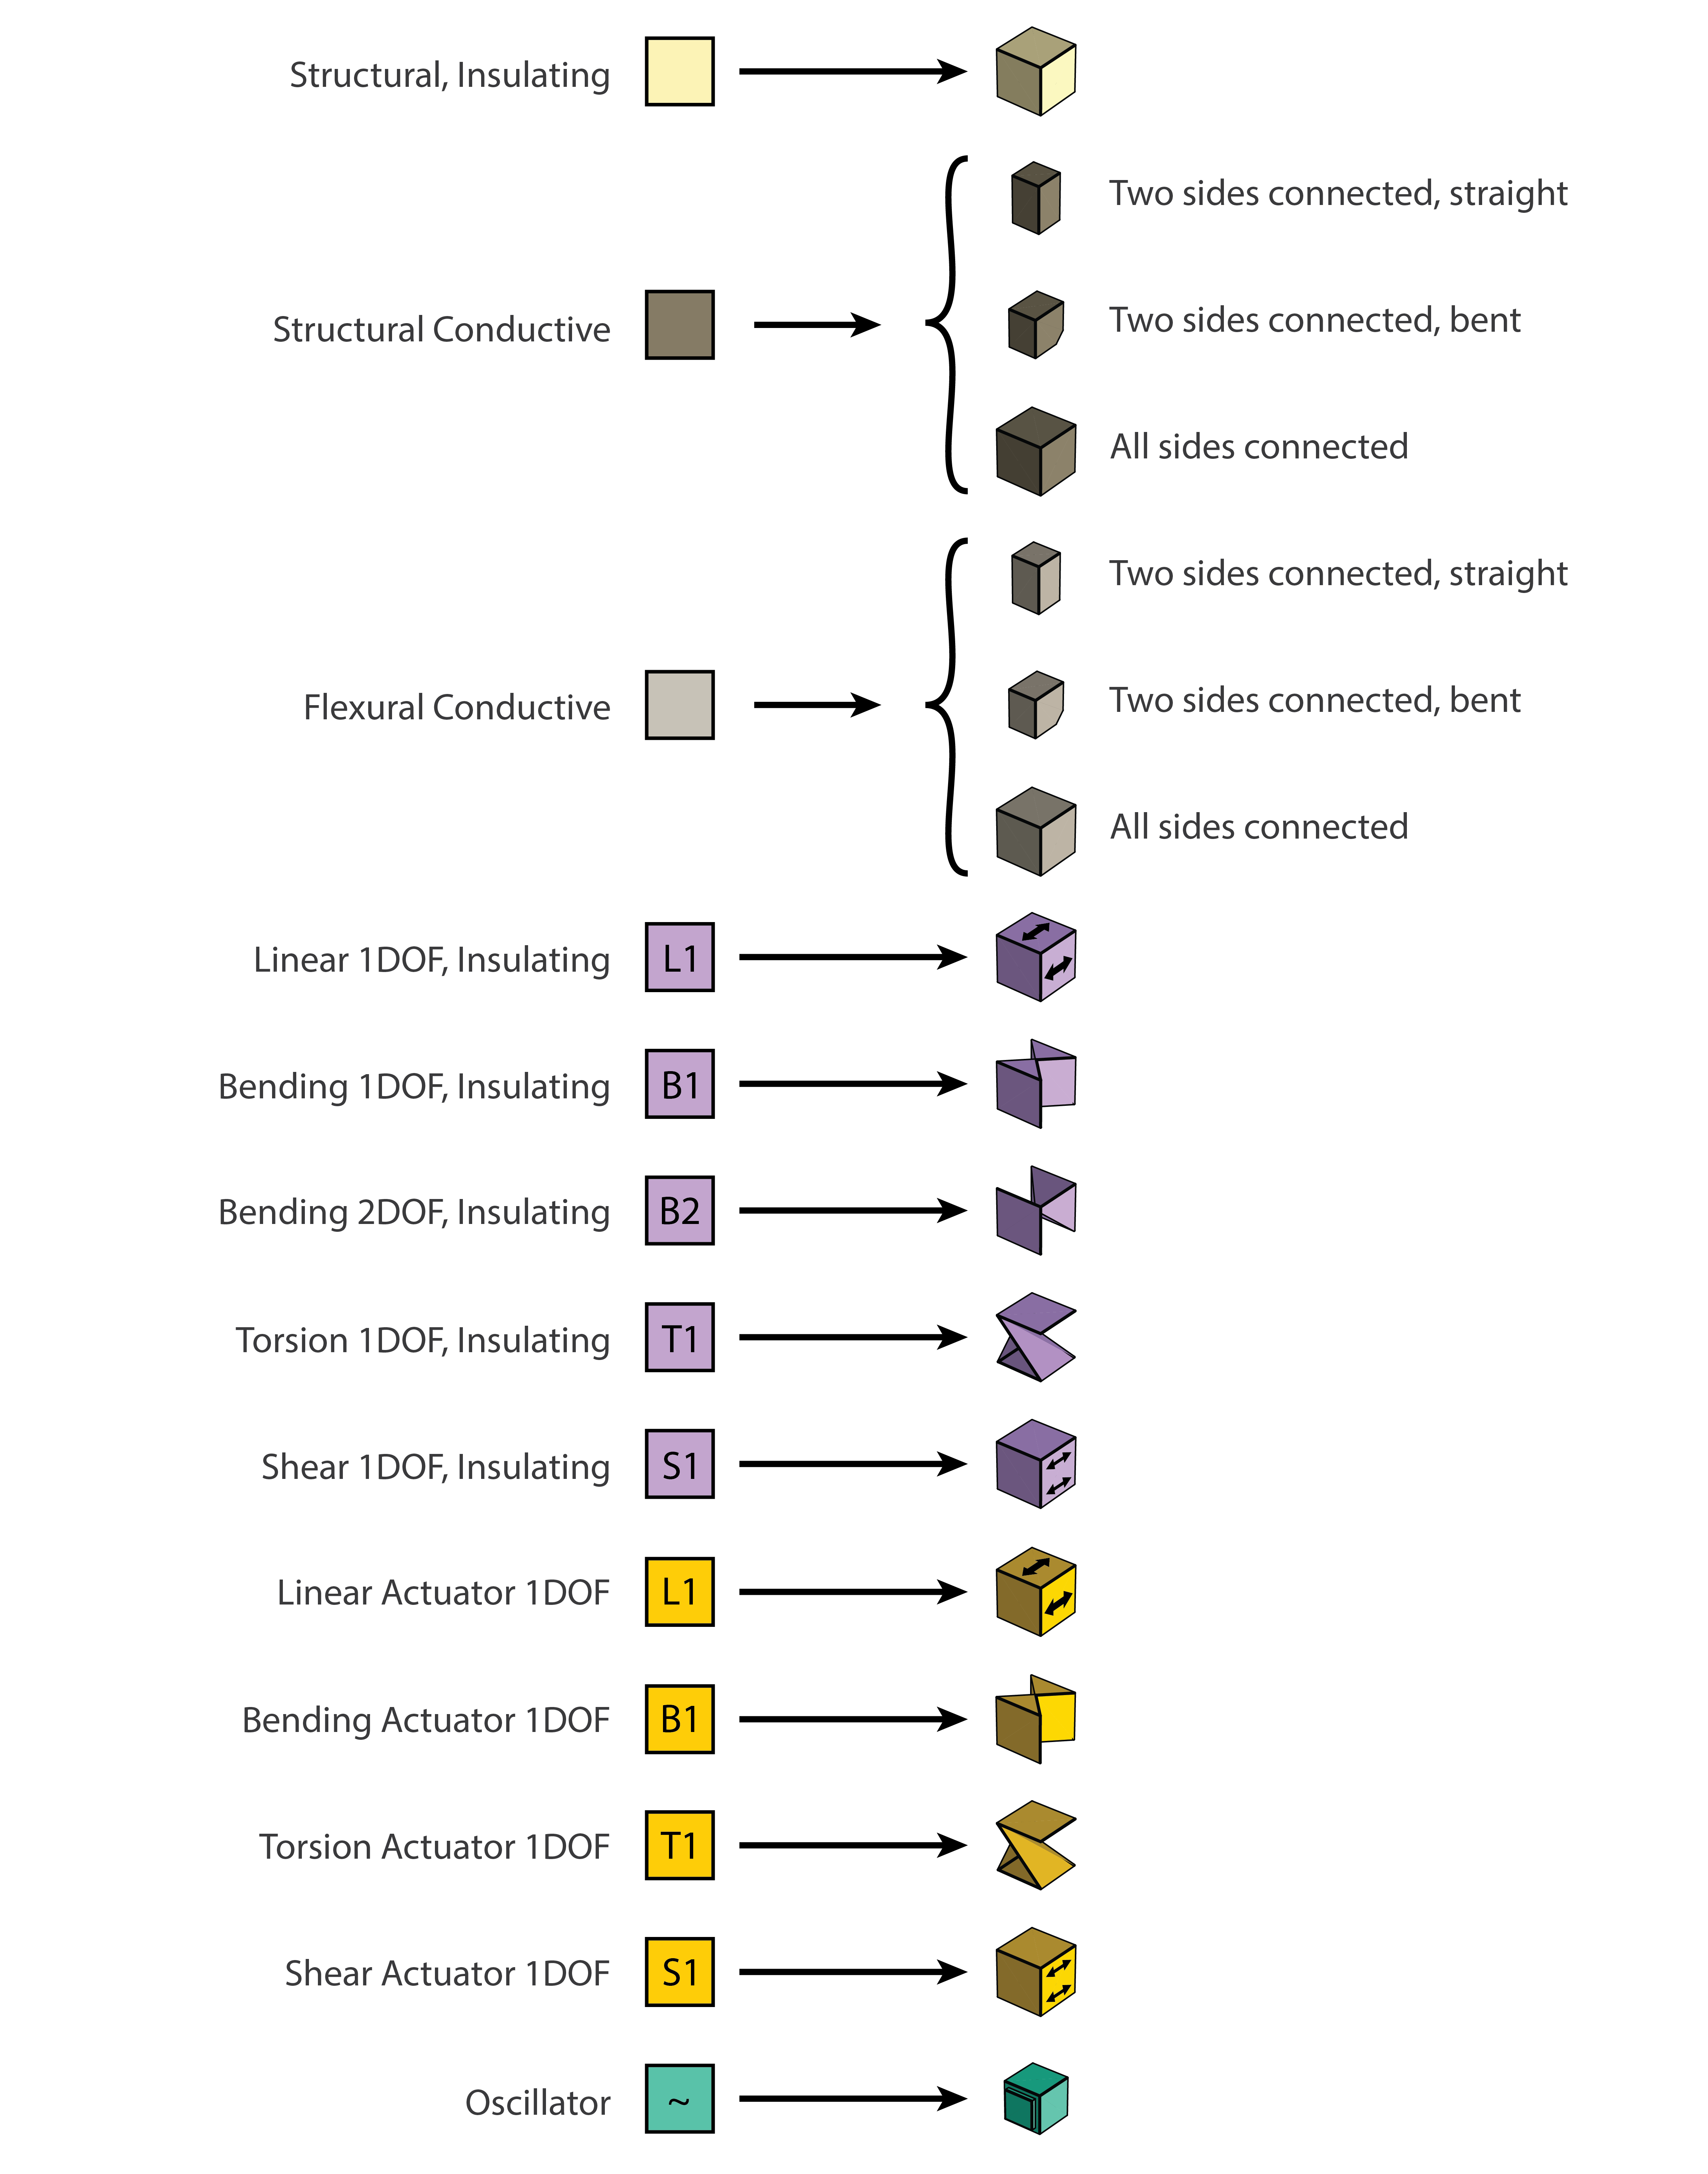
\includegraphics[width=\linewidth]{cellMeshes.png}
  \caption{Meshes and textures used to represent different material types and convey the orientation of anisotropic cells.}
  \label{fig:cellMeshes}
\end{figure}

\section{GUI}

AmoebaCAD borrows most of its GUI from DMDesign (Chapter \ref{chap:CAD}), with a few exceptions.  A cell rotation interface (Figure \ref{fig:rotationGUI}) allows users to rotate cells in 3D, so anisotropic cells may be oriented in any direction.  These cell rotations are saved as JSON when the assembly is saved.  A 3D selection tool allows users to select large rectangular regions of space to fill with material, cut away material, and clone or mirror an existing structure into another region (Figure \ref{fig:selectiontoolGUI}).\\

Anisotropic cells in AmoebaCAD are represented graphically with special meshes, illustrated in Figure \ref{fig:cellMeshes}.  Some cells (e.g. the straight and bent conducting cells) appear to occupy a smaller volume than other cells, but this is meant only as a visualization of their special properties.  All cells fill the same volume and are joined mechanically with six face-connected neighbors.

\section{GPU Programming}

JavaScript is loosely typed and therefore not an especially fast language out of the box.  Most modern web browsers support Just In Time (JIT) compilation of JavaScript code, which helps make it competitive with compiled languages.  Storing large datasets in typed arrays also helps to speedup array access and operations at runtime \cite{Network}.\\

During the development of AmoebaCAD, I found that typed arrays were not giving my app the performance I was looking for, so I began running the bulk of the math involved in the physics engine on the GPU.  

Mathematical programming on the GPU through WebGL is a loosely supported "hack" at the current state of writing this thesis.  Data is passed to the GPU cores as 2D arrays - image textures that would normally be used for WebGL rendering.  Though normal GL rending would only necessitate byte arrays (uInt8), WebGL also supports Int8/16/32, uInt16/32 and Float32 textures.
A concise reference for the current WebGL standards is provided by the Khronos Group \cite{Group}.
\\

Computing in the GPU does create some hardware dependencies for this application that would not have otherwise been present.  For example, some GPUs have a hard limit of 8 textures that can be loaded into memory and accessed by each GPU core at a time.  In this case I've implemented a back up \href{https://developer.mozilla.org/en-US/docs/Web/JavaScript/Typed_arrays}{typed array} engine that should be supported by all hardware configurations.

\begin{figure}
  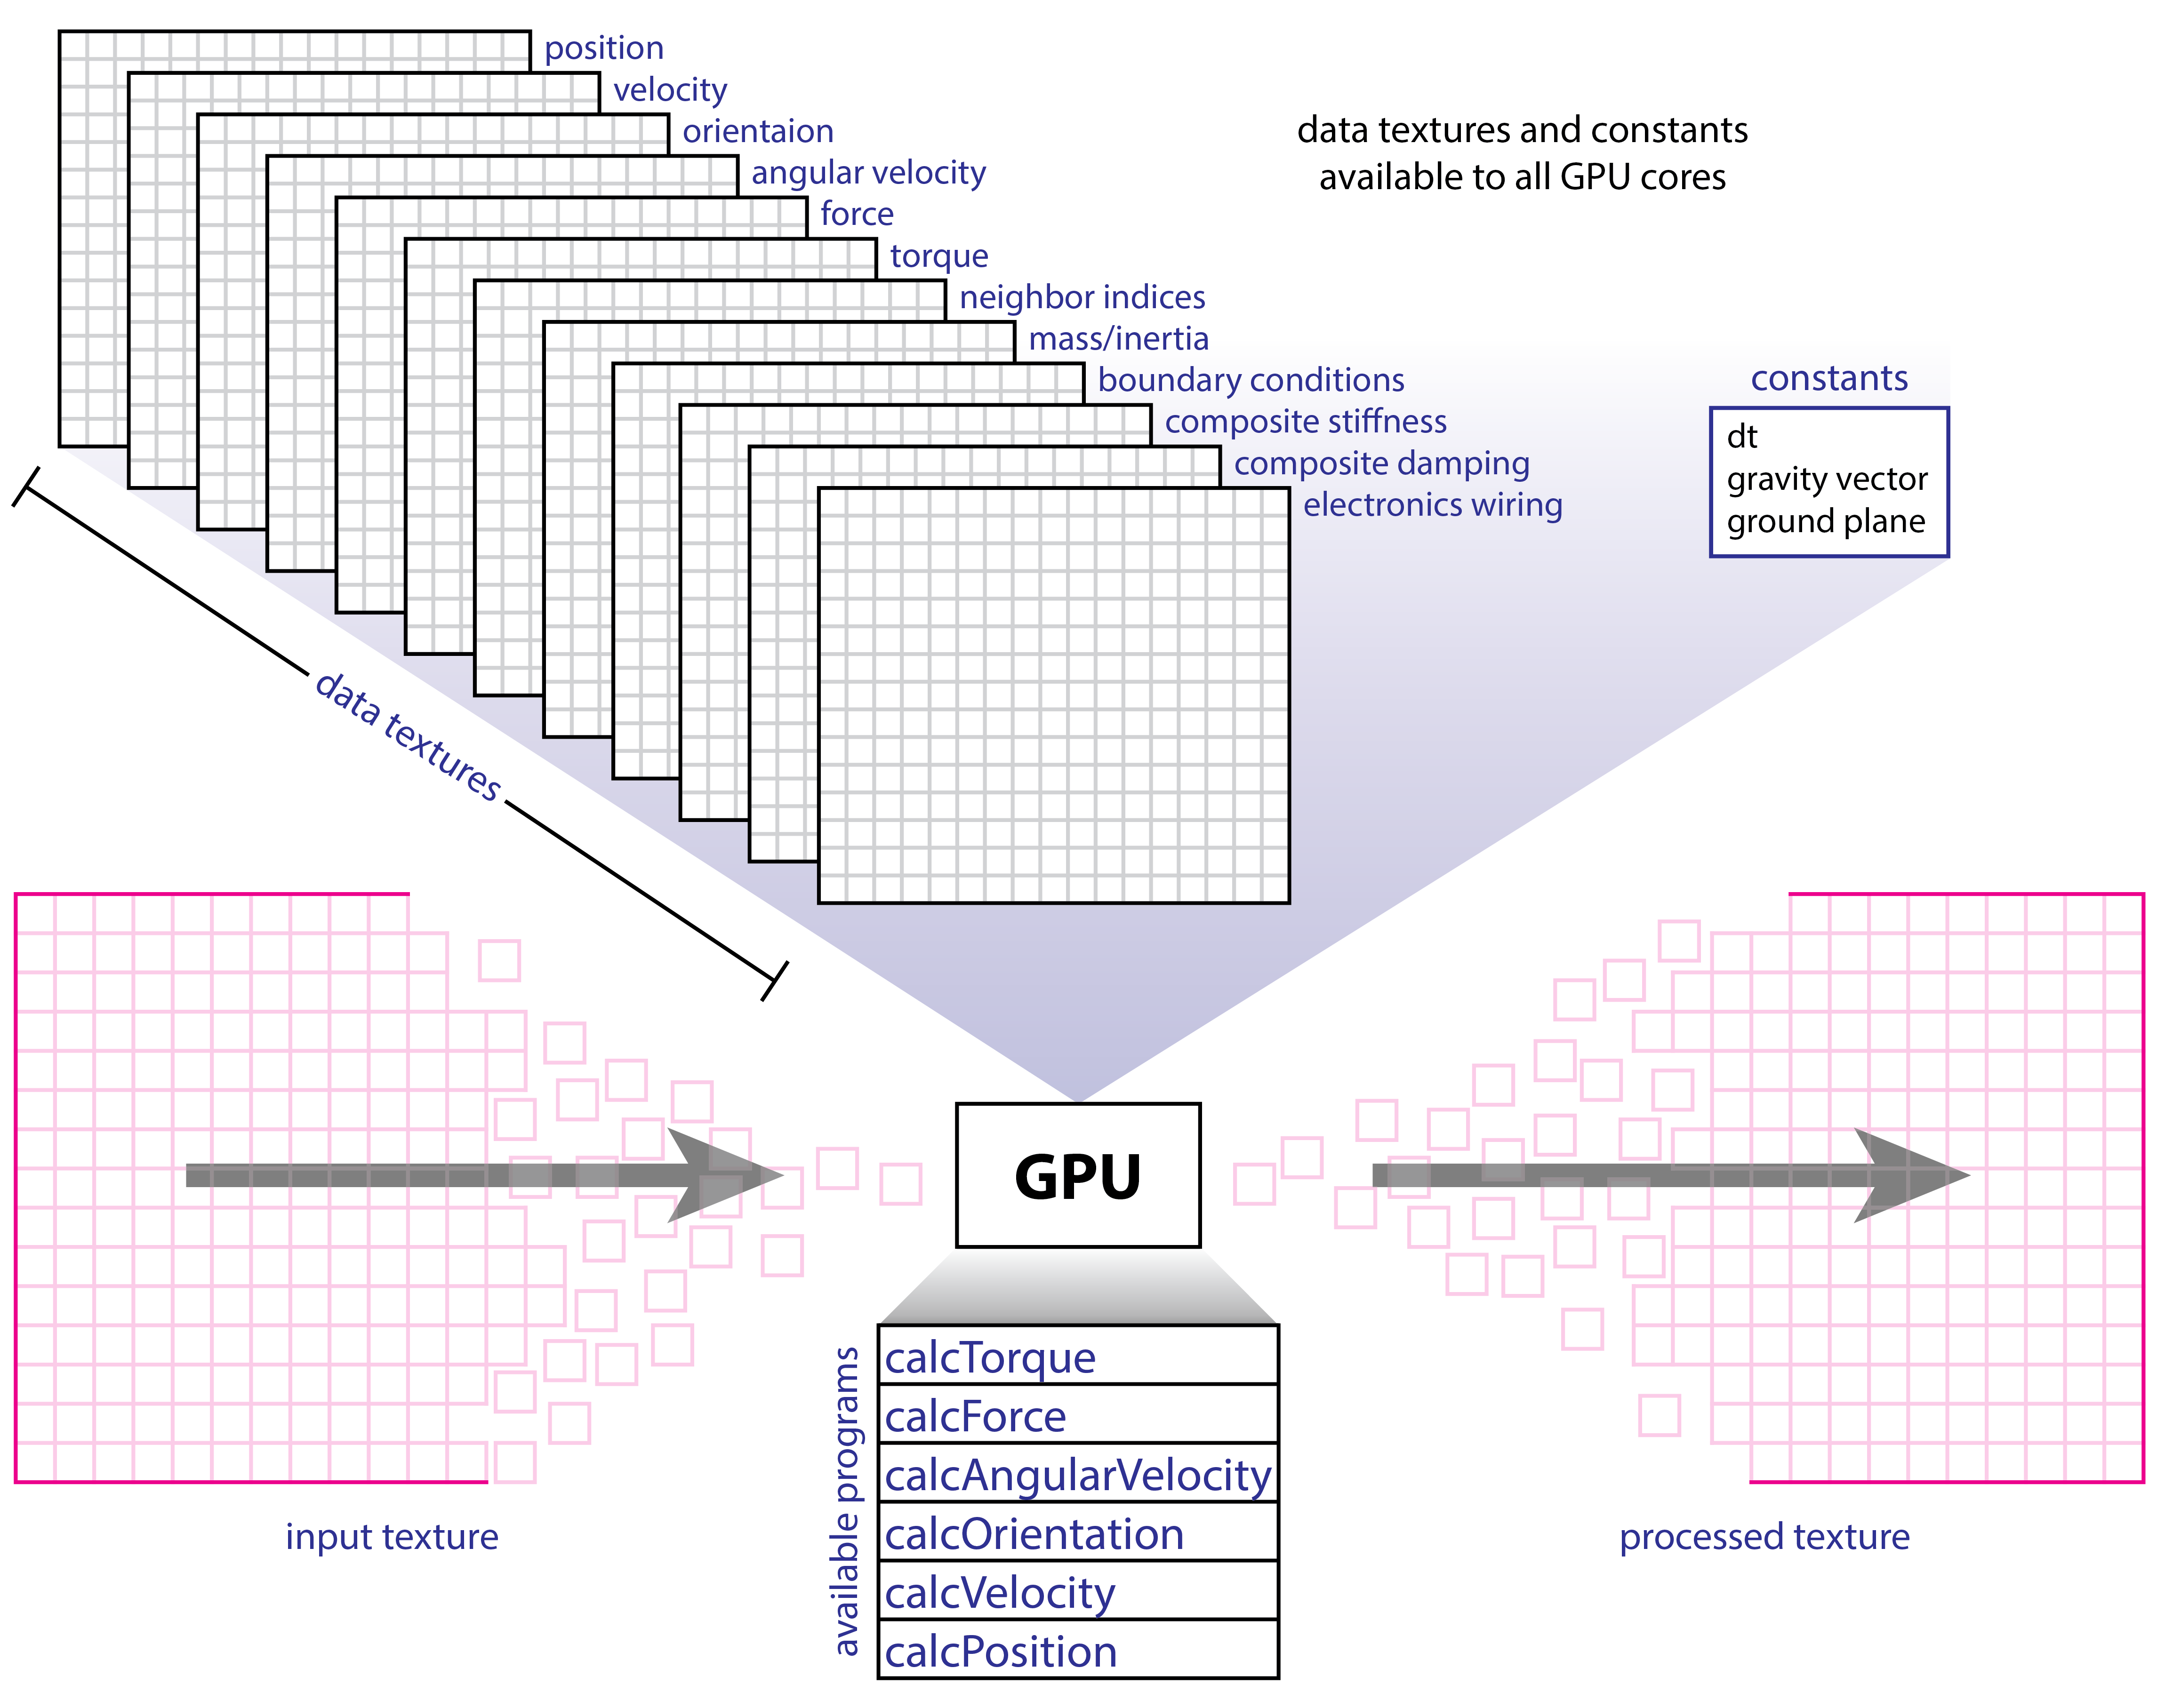
\includegraphics[width=\linewidth]{gpuprogramming.png}
  \caption{}
  \label{fig:gpuprogramming}
\end{figure}


\section{Other Performance Speedups}

Additional speedups in mathematical operations increase runtime speed of the code.  As demonstrated in Chapter \ref{chap:functionSim}, the math behind the mechanical modeling involves liberal use of quaternions.  An efficient method of applying quaternions to vectors is given below:\\

\[ t = 2 \left[ \begin{array}{ccc}
q_x\\
q_y\\
q_z
 \end{array} \right] \times v\]
\[ v_{rotated} = v + q_wt +  \left[ \begin{array}{ccc}
q_x\\
q_y\\
q_z
 \end{array} \right] \times t\]
 
 This method uses fewer floating point operations than the standard Hamilton product from equation \ref{eq:hamiltonprod} \cite{Reinalter}.\\
 
 AmoebaCAD is still very much under development and is not ready for rigorous optimization at this time.  In the coming months I will integrate the methods above into the codebase.

\section{Numerical Instability}

\begin{figure}
  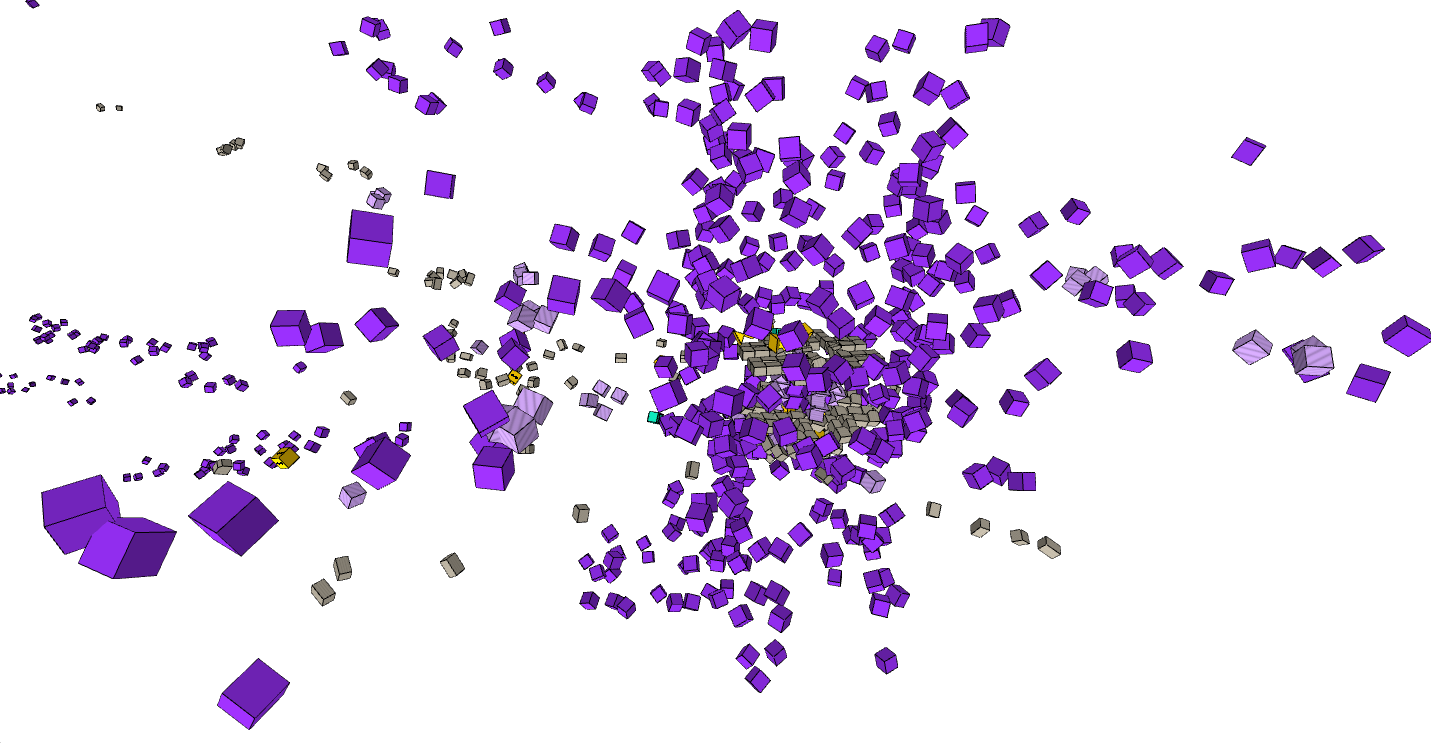
\includegraphics[width=\linewidth]{instability.png}
  \caption{instability.png.}
  \label{fig:instability}
\end{figure}

\section{Examples}
